\documentclass[a4paper,12pt]{article}

\usepackage[brazil]{babel}
\usepackage[utf8]{inputenc}
\usepackage{graphicx}

\author{Carlos Brandt}
\title{Aprendizagem de M\'aquina - Primeira lista de exerc\'icios}

\begin{document}
\maketitle

\section*{Regress\~ao Linear 1: {\small {\tt reg\_1\_tr\_X.dat, reg\_1\_tr\_Y.dat, reg\_1\_ts\_X.dat}}}

Os pontos do conjunto de treinamento do primeiro problema de regress\~ao podem ser vistos na figura abaixo.

\begin{figure}[!h]
	\centering
	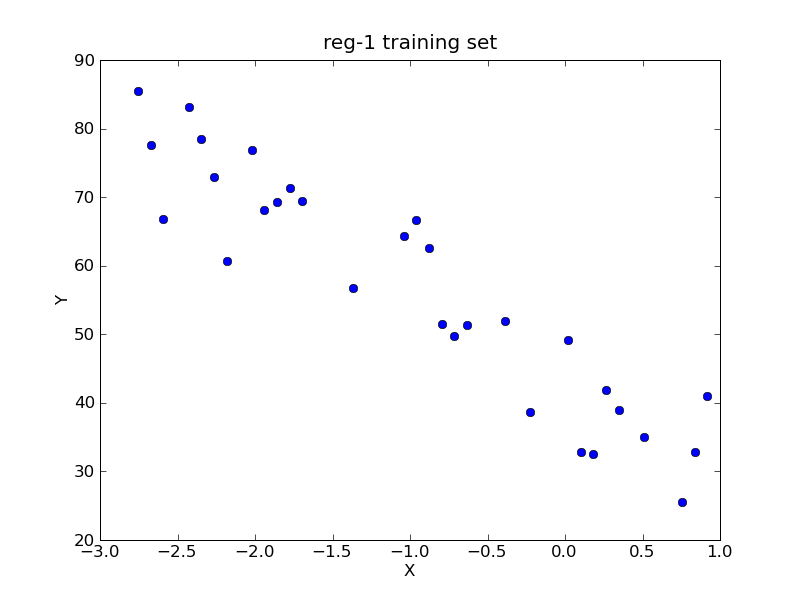
\includegraphics[scale=0.5]{reg_1_plot.png}
\end{figure}

Podemos observar que os pontos se distribuem como que ao longo e arredores de uma reta, ou seja, um \'otimo ajuste para este conjunto de dados seria uma reta no meio dos pontos graficados.

Observado isto, opto por utilizar o modelo de regress\~ao linear para ajustar uma reta sobre a distribui\c c\~ao de pontos.

Aplicando regress\~ao linear ao ajuste dos pontos, obtemos um resultado com erro quadr\'atico m\'edio,
$$ \frac{1}{m}\sum_{i=1}^{m} \Big( y_{fit}(i) - y(i) \Big) = 37.27, $$
onde $y_{fit}(i)$ constitui o resultado do ajuste para cada ponto $x(i)$ do conjunto de tamanho $m$.

A curva ajustada para os pontos do conjunto "1" tem a seguinte forma:
$$ y_{fit} = -13.68 x + 43.23$$
i.e,
$$\vec \theta = [43.23 , -13.68]$$

O resultado da regress\~ao pode ser visto na figura que segue,
\begin{figure}[!h]
	\centering
	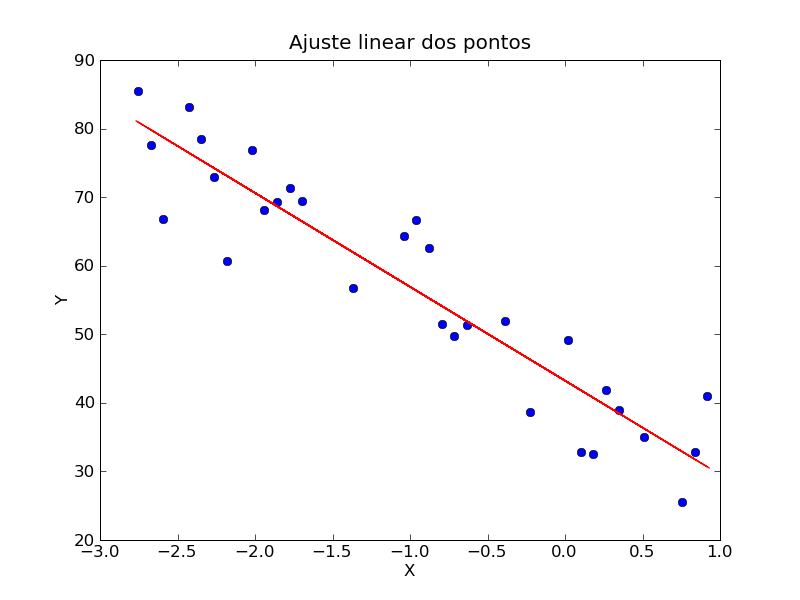
\includegraphics[scale=0.5]{reg_1_plot_reglin.png}
	\caption{Ajuste linear dos pontos apresentados.}
\end{figure}

O procedimento foi realizado com os tr\^es algor\'itmos de minimiza\c c\~ao dados em aula: descida pelo gradiente em lote, descida pelo gradiente estoc\'astico e m\'inimos quadrados. S\~ao estes apresentados a seguir:

\begin{verbatim}
# Descida em Lote:
    while( diff > eps ):
        inn = (x * theta);
        J[:] = y[:] - inn[:];
        Jm = np.sum(J);
        for j in xrange(0,n):
            theta[j] += alpha * (( J.T * x ).T)[j];
    
        # Estima-se o desvio da parametrizacao relativo aos dados.
        tc = np.sum([ i**2 for i in theta ])**0.5;
        diff = abs( tc - tp );
        tp = tc;
---
    
#Descida Estoc\'astica:
    while( diff > eps ):
        for i in xrange(0,m):
            for j in xrange(0,n):
                J =  y[i] - x[i] * theta;
                theta[j] += alpha * ( J * (x[i].T)[j] );

        # Estima-se o desvio da parametrizacao relativo aos dados.
        tc = np.sum([ i**2 for i in theta ])**0.5;
        diff = abs( tc - tp );
        tp = tc;
---
    
# M\'inimos quadrados:
    Xprod = x.T * x;
    Xinv = Xprod.I;
    Xprod = Xinv * x.T;

    theta = Xprod * y;
---
%yfit teste:    
%array([ 65.31098484,  59.72324345,  35.1371813 ,  44.07756753,
%        72.01627452,  34.01963302,  29.5494399 ,  47.43021237,
%        84.30930559,  64.19343656,  63.07588828,  45.19511581,
%        37.37227785,  77.60401592,  83.19175732,  82.07420904,
%        58.60569517,  60.84079172,  49.66530893,  50.78285721])

\end{verbatim}

\end{document}
